\documentclass[12pt,a4paper]{article}
\usepackage{cmap} % Makes the PDF copiable. See http://tex.stackexchange.com/a/64198/25761
\usepackage[T1]{fontenc}
\usepackage[brazil]{babel}
\usepackage[utf8]{inputenc}
\usepackage{amsmath}
\usepackage{amsfonts}
\usepackage{amssymb}
\usepackage{amsthm}
\usepackage{textcomp} % \degree
\usepackage{gensymb} % \degree
\usepackage[usenames,svgnames,dvipsnames]{xcolor}
\usepackage{hyperref}
\usepackage{multicol}
\usepackage{graphicx}
\usepackage[margin=2cm]{geometry}
\usepackage{systeme}

\hypersetup{
    colorlinks = true,
    allcolors = {blue}
}

% TODO: Consider using exsheets
% http://linorg.usp.br/CTAN/macros/latex/contrib/exsheets/exsheets_en.pdf
%
% http://ctan.org/tex-archive/macros/latex/contrib/exercise/
% Options: answerdelayed,lastexercise,noanswer
\usepackage[answerdelayed,lastexercise]{exercise}

\addto\captionsbrazil{%
\def\listexercisename{Lista de exerc\'icios}%
\def\ExerciseName{Exerc\'icio}%
\def\AnswerName{Solu\c{c}\~ao do exerc\'icio}%
\def\ExerciseListName{Ex.}%
\def\AnswerListName{Solu\c{c}\~ao}%
\def\ExePartName{Parte}%
\def\ArticleOf{de\ }%
}

\renewcommand{\ExerciseHeaderTitle}{(\ExerciseTitle)\ }
\renewcommand{\ExerciseListHeader}{%\ExerciseHeaderDifficulty%
\textbf{%\ExerciseListName\
\ExerciseHeaderNB.\ %
%\ --- \ 
\ExerciseHeaderTitle}%
%\ExerciseHeaderOrigin
\ignorespaces}
\renewcommand{\AnswerListHeader}{\textbf{\ExerciseHeaderNB.\ (\AnswerListName)\ }}

\newcommand*\tg{\operatorname{tg}}

\newcommand*\R{\mathbb{R}}

\renewcommand{\theenumi}{\alph{enumi}}
\renewcommand\labelenumi{(\theenumi) }

\newcommand*\tipo{Prova I}
\newcommand*\turma{PRO112-04U}
\newcommand*\disciplina{CAN0001}
\newcommand*\eu{Helder G. G. de Lima}
\newcommand*\data{04/04/2017}

\author{\eu}
\title{\tipo - \disciplina}
\date{\data}

\begin{document}
\thispagestyle{empty}
\newgeometry{margin=2cm,bottom=0.5cm}
\begin{center}

\includegraphics[width=9.0cm]{marca} \\
\textbf{\tipo\ (\disciplina / \turma)} \\
Prof. \eu\footnote{
Este é um material de acesso livre distribuído sob os termos da licença \href{https://creativecommons.org/licenses/by-sa/4.0/deed.pt_BR}{Creative Commons Atribuição-CompartilhaIgual 4.0 Internacional}}
\end{center}

\noindent Nome do(a) aluno(a): \underline{\hspace{9,7cm}} Data: \underline{\data}

%\section*{Instruções}
\begin{center}\fbox{
\begin{minipage}{14cm}

{\footnotesize
\begin{itemize}
\renewcommand{\theenumi}{\Roman{enumi}}
\item Identifique-se em todas as folhas.
\item Mantenha o celular e os demais equipamentos eletrônicos desligados durante a prova.
\item Justifique cada resposta com cálculos ou argumentos baseados na teoria estudada.
\item Escreva todos os números usados nos cálculos com 5 dígitos após a vírgula.
\item Resolva apenas os itens de que precisar para somar 10,0 pontos.
\end{itemize}
}

\end{minipage}
}
\end{center}

%\section*{Questões}
\begin{ExerciseList}

\Exercise[title={1,0}]
Descreva em detalhe a motivação geométrica de algum dos métodos estudados, mostrando como é calculada a aproximação $x_k$ a partir de $x_{k-1}$ e da função $f$.
\Answer
Estas são as motivações geométricas dos métodos estudados:
\begin{enumerate}
\item \textbf{Bissecção}: Em cada iteração, o método parte de um intervalo fechado que contém alguma raiz da função, divide-o exatamente ao meio e escolhe para a próxima etapa um subintervalo no qual ainda exista uma raiz (a escolha é feita com base no teorema de Bolzano, que garante a existência de uma raiz quando uma função contínua $f$ tem sinais diferentes nos extremos do intervalo). O comprimento dos intervalos considerados vai sendo reduzido pela metade a cada iteração, e com isso é possível se aproximar de uma raiz tanto quanto for necessário, desde que seja feito um número suficientemente grande de iterações.
\item \textbf{Posição falsa}: Como na bissecção, a cada iteração subdivide-se um intervalo fechado que contém a raiz em dois subintervalos, e escolhe-se um deles para uso na próxima iteração. O que muda é o ponto em que é feita a divisão: em vez de usar sempre o ponto médio dos extremos do intervalo $[a,b]$, é feita uma média ponderada dessas extremidades, levando em conta o valor de $f$ em cada uma. Geometricamente, isso corresponde a ligar os pontos $(a, f(a))$ e $(b, f(b))$ por uma reta, e encontrar a interseção desta com o eixo horizontal.
\item \textbf{Iteração de ponto fixo}: Neste método a equação $f(x) = 0$ é trocada por uma equação equivalente da forma $\varphi(x) = x$, de modo que as raízes de $f$ sejam exatamente os pontos fixos de $\varphi$. Assim, em vez de procurar uma interseção entre o gráfico de $f$ e o eixo horizontal, o objetivo passa a ser a busca de uma interseção entre o gráfico de $\varphi$ e a bissetriz do primeiro e do terceiro quadrantes, que é a reta $y = x$. Na melhor das hipóteses, a aplicação de $\varphi$ repetidas vezes a um valor inicial $x_0$, produz uma sequência de aproximações $\{ x_k \}_{k=0}^\infty$, com $x_k = \varphi( x_{k-1} )$, que converge para um ponto fixo de $\varphi$.
\item \textbf{Newton-Raphson}: Este é um caso particular do método de iteração de ponto fixo, em que a função $\varphi$ é escolhida pensando em acelerar a convergência. Geometricamente, dada uma aproximação $x_{k-1}$, a função $\varphi$ produz o ponto $x_k = \varphi( x_{k-1} )$ que é obtido ao intersectar o eixo horizontal com a reta tangente ao gráfico de $f$ no ponto $(x_{k-1}, f(x_{k-1}))$. Em outras palavras, assume-se que nas vizinhanças de uma raiz $\overline{x}$ de $f$, ela é diferenciável e sua aproximação por uma função afim tem uma raiz que é uma boa aproximação de $\overline{x}$.
\item \textbf{Secante}: Neste método, evita-se o uso da derivada de $f$ que é necessária no método de Newton-Rhapson (para obter a inclinação da reta tangente ao gráfico de $f$), calculando-se uma estimativa desta derivada em $x_{k-1}$. Isso é feito considerando que quando duas iterações consecutivas $x_{k-2}$ e $x_{k-1}$ estão suficientemente próximas, a reta secante ao gráfico de $f$ nos pontos $A = (x_{k-2}, f(x_{k-2}))$ e $B = (x_{k-1}, f(x_{k-1}))$ tem uma inclinação próxima da inclinação da reta tangente no ponto $(x_{k-1}, f(x_{k-1}))$. Assim, a partir destas duas iterações, obtem-se $x_k$ como a interseção do eixo horizontal com a reta secante ao gráfico de $f$ em $A$ e $B$.
\end{enumerate}

\Exercise%[title={2,0}]
O polinômio $p(x) = x^3 - x^2 - x + 1$ tem raízes $r_0 = -1$ e $r_1 = r_2 = 1$ no intervalo $[-2, 3]$.
\begin{enumerate}
\item \textbf{(1,0)} Se for aplicado o método da bissecção com intervalo inicial $[-2, 3]$, o método convergirá para qual das raízes? Justifique.
\item \textbf{(1,0)} Se o intervalo inicial for $[-2,3]$, em quantas iterações o erro absoluto será $\varepsilon_a < 10^{-2}$?
\item \textbf{(1,0)} Pode-se obter a outra raiz por este método? E pelo método da posição falsa?
\end{enumerate}
\Answer

\begin{enumerate}
\item Como $f(-2) = -9 < 0$ e $f(3) = 16 > 0$, é garantido que o método da bissecção convergirá para alguma raiz pertencente a $(-2, 3)$. O intervalo inicial é dividido ao meio, no ponto $x_0 = \frac{-2 + 3}{2} = \frac{1}{2} =0{,}5$, e como $f(x_0) = \frac{3}{8} = 0,375 > 0$, utiliza-se o intervalo $\left[-2, \frac{1}{2} \right]$ na próxima iteração. Assim, o método converge para a raiz $-1$, que está neste intervalo.
\item A quantidade $k$ de iterações deve satisfazer
$
k
> \frac{\log(b_0 - a_0) - \log(\varepsilon_a)}{\log(2)}
= \frac{\log(5) - \log(10^{-2})}{\log(2)}
\approx 8,97,
$
ou seja, é preciso 9 iterações.

Outra forma de chegar à mesma conclusão é lembrar que o comprimento dos intervalos são reduzidos pela metade a cada iteração, então:
\begin{center}
\begin{tabular}{|c|c|c|c|c|c|c|c|c|c|c|}
\hline
$k$ & $0$ & $1$ & $2$ & $3$ & $4$ & $5$ & $6$ & $7$ & $8$ & $9$ \\
\hline
$\varepsilon$ & $5$ & $2,5$ & $1,25$ & $0,625$ & $0,3125$ & $0,15625$ & $0,07813$ & $0,03907$ & $0,01953$ & $0,00977$ \\
\hline
\end{tabular}
\end{center}

Também seria possível, e mais trabalhoso, executar todas as iterações até que a distância entre $x_k$ e a raiz $r_0 = -1$ fosse menor do que $10^{-2}$:
\begin{center}
\begin{tabular}{|r|r|r|r|r|r|}
\hline
$k$ &  $a_k$ &  $b_k$ & $x_k = \frac{a_k+b_k}{2}$ & $b_k - a_k$ & $f(x_k)$ \\
\hline
0 & -2,00000 &  3,00000 &  0,50000 & 5,00000 &  0,37500 \\
\hline
1 & -2,00000 &  0,50000 & -0,75000 & 2,50000 &  0,76563 \\
\hline
2 & -2,00000 & -0,75000 & -1,37500 & 1,25000 & -2,11523 \\
\hline
3 & -1,37500 & -0,75000 & -1,06250 & 0,62500 & -0.26587 \\
\hline
4 & -1,06250 & -0,75000 & -0,90625 & 0,31250 &  0,34067 \\
\hline
5 & -1,06250 & -0,90625 & -0,98437 & 0,15625 &  0,06155 \\
\hline
6 & -1,06250 & -0,98437 & -1,02344 & 0,07813 & -0,09597 \\
\hline
7 & -1,02344 & -0,98437 & -1,00390 & 0,03907 & -0,01566 \\
\hline
8 & -1,00390 & -0,98437 & -0,99413 & 0,01953 &  0,02334 \\
\hline
9 & -1,00390 & -0.99413 & \textbf{-0,99901} & 0,00977 &  0,00396 \\
\hline
\end{tabular}
\end{center}

\item Como as raízes são $r_0 = -1$ e $r_1 = r_2 = 1$, tem-se $p(x) = (x+1)(x-1)^2$ e portanto:
\begin{center}
\begin{tabular}{|c|c|c|c|c|c|}
\hline
$x$ & $(-\infty, -1)$ & $-1$ & $(-1, +1)$ & $1$ & $(+1, +\infty)$ \\
\hline
$f(x)$ & $-$ & $0$ & $+$ & $0$ & $+$ \\
\hline
\end{tabular}
\end{center}
Em particular, para valores próximos de $r_1 = r_2 = 1$, $f$ sempre é positiva, e não há como obter um intervalo $[a,b]$ pequeno (por exemplo, com $|b - a| < 1/10$), contendo esta raiz, no qual $f$ mude de sinal. Sem isso, não é possível garantir a convergência do método da bissecção para este zero de $f$. O método da posição falsa tem o mesmo problema.
\end{enumerate}

\Exercise%[title={2,0}]
Seja $f: \R \to \R$ a função definida por $f(x) = e^{-x} - 2x + 3$.
\begin{enumerate}
\item \textbf{(0,5)} Esboce o gráfico de $f$ e, a partir dele, obtenha uma estimativa $x_0$ da raiz de $f$.
\item \textbf{(1,5)} Para cada uma das funções de iteração a seguir explique (sem calcular as iterações) se há ou não garantia de convergência para a raiz de $f$:
\begin{multicols}{3}
\begin{enumerate}
\item $\varphi_1(x) = (e^{-x}+3)/2$
\item $\varphi_2(x) = e^{-x}-x+3$
\item $\varphi_3(x) = -\ln{(2x-3)}$
\end{enumerate}
\end{multicols}
\item \textbf{(2,0)} Aplique o método de iteração de ponto fixo usando uma das funções acima (para a qual tenha garantido a convergência) para obter uma raiz com erro absoluto $\varepsilon_a < 0.0001$. Indique os valores de $x_k$, $f(x_k)$ e $|x_k - x_{k-1}|$ a cada iteração.
\end{enumerate}
\Answer
\begin{enumerate}
\item
\begin{minipage}[c]{0.50\textwidth}
Observando-se que
$f(0) = 4$,
$f(1) \approx  1.36788$,
$f(2) \approx -0.86466$ e
$f(3) \approx -2.95021$
o esboço deverá parecido com o da figura ao lado.

Como a função muda de sinal em $[1, 2]$, pode-se escolher como estimativa inicial valores como $x_0 = 1,5$, ou $x_0 = 1,7$, etc que pertencem a este intervalo, dependendo do que for apropriado para a função de iteração escolhida.
\end{minipage}
\begin{minipage}[c]{0.25\textwidth}
  \centering
  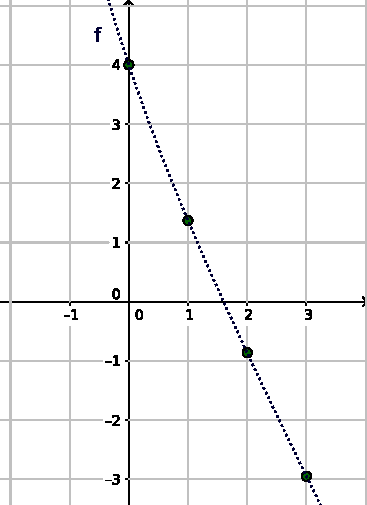
\includegraphics[width=3.78cm]{img/prova-1-pro-3a-plot.pdf}
\end{minipage}

\item 
\begin{enumerate}
\item Se $\varphi_1(x) = (e^{-x}+3)/2$, então $\varphi_1^\prime(x) = \dfrac{-e^{-x}}{2}$ é contínua em $\R$. Além disso,
\[
| \varphi_1^\prime(x) | < 1
\Leftrightarrow
\left| -e^{-x}/2 \right| < 1
\Leftrightarrow
e^{-x} < 2
\Leftrightarrow
x > -\ln(2) \approx -0.69315.
\]
Então para qualquer aproximação inicial $x_0 \in (-\ln(2), +\infty)$, o método de iteração do ponto fixo converge, se for utilizada a função de iteração $\varphi_1$.
\item Para a função $\varphi_2(x) = e^{-x}-x+3$ tem-se $\varphi_2^\prime(x) = -e^{-x}-1$, que é contínua. Assim,
\[
| \varphi_2^\prime(x) | < 1
\Leftrightarrow
\left| -e^{-x}-1 \right| < 1
\Leftrightarrow
\left| e^{-x} + 1 \right| < 1.
\]
Como $e^{-x} > 0$, a desigualdade acima não se verifica para nenhum $x \in \R$, e portanto não há garantia de que a sequência gerada pelo método da iteração de ponto fixo converge para a uma raiz, qualquer que seja a aproximação inicial $x_0$ escolhida.
\item Considerando $\varphi_3(x) = -\ln{(2x-3)}$ com domínio $(3/2, +\infty)$, tem-se que tanto $\varphi_3$ quanto $\varphi_3^\prime(x) = \dfrac{-2}{2x-3}$ são contínuas. No entanto, para $x > 3/2$,
\[
| \varphi_3^\prime(x) | < 1
\Leftrightarrow
\left| \dfrac{-2}{2x-3} \right| < 1
\Leftrightarrow
2 < |2x-3| = 2x-3
\Leftrightarrow
x \in \left(5/2, +\infty \right).
\]
\end{enumerate}
Em particular, $|\varphi_3^\prime(x)| > 1$ para todo $x \in \left(3/2, 5/2 \right] = \left(1,5, 2,5 \right]$. Logo, não existe um intervalo fechado $I$ contendo a raiz, no qual há garantia de convergência para uma raiz.

\item Usando a função de iteração $\varphi_1$, gera-se uma sequência $(x_k)_{k=0}^\infty$ que converge para uma raiz de $f$, na qual $x_0 = 3/2$ e $x_k = (e^{-x_{k-1}}+3)/2$ para $k \geq 1$. Estes são os resultados das 5 primeiras iterações do método, arredondados no quinto dígito decimal a cada iteração:
\begin{center}
\begin{tabular}{|r|r|r|r|r|}
\hline
$k$ &  $x_{k-1}$ &  $x_k$ & $|x_k - x_{k-1}|$ & $f(x_k)$ \\
\hline
0 &       - & 1.50000 &      -  &  0.22313 \\
\hline
1 & 1.50000 & 1.61157 & 0.11157 & -0.02357 \\
\hline
2 & 1.61157 & 1.59979 & 0.01178 &  0.00236 \\
\hline
3 & 1.59979 & 1.60097 & 0.00118 & -0.00024 \\
\hline
4 & 1.60097 & 1.60085 & 0.00012 &  0.00002 \\
\hline
5 & 1.60085 & \textbf{1.60086} & 0.00001 &  0,00000 \\
\hline
\end{tabular}
\end{center}

Como $|x_5 - x_4| \approx 0.00001 < 0.0001$, conclui-se que $x_5 = 1.60086$ é uma aproximação de uma raiz de $f$ com a precisão desejada.
\end{enumerate}

\Exercise[title={2,0}]
Utilize 5 iterações do método da secante para obter uma aproximação da menor raiz positiva de $f(x) = \tg(x) - x$, sabendo que ela está no intervalo $I = [4.4, 4.6]$, e estime o erro absoluto cometido. Escreva os valores de $x_k$, $f(x_k)$ e $|x_k - x_{k-1}|$ a cada iteração.%obtidos na $k$-ésima iteração.
\Answer
Estas são as 5 primeiras iterações do método da secante com aproximações iniciais $x_{-1} = 4.4$ e $x_{0} = 4.6$, com arredondamento no quinto dígito decimal a cada iteração:

\begin{center}
\begin{tabular}{|r|r|r|r|r|}
\hline
$k$ &  $x_{k-1}$ &  $x_k$ & $|x_k - x_{k-1}|$ & $f(x_k)$ \\
\hline
-1 &       - & 4.40000 & - & -1.30368 \\
\hline
 0 & 4.40000 & 4.60000 & 0.20000 & 4.26017 \\
\hline
 1 & 4.60000 & 4.44686 & 0.15314 & -0.76972 \\
\hline
 2 & 4.44686 & 4.47029 & 0.02343 & -0.42076 \\
\hline
 3 & 4.47029 & 4.49854 & 0.02825 & 0.10616 \\
\hline
 4 & 4.49854 & 4.49285 & 0.00569 & -0.01127 \\
\hline
 5 & 4.49285 & \textbf{4.49340} & 0.00055 & -0.00019 \\
\hline
\end{tabular}
\end{center}
\medskip
Nesta etapa, obtém-se a aproximação $x_5 = 4.49340$, com erro $\varepsilon_a = |x_5 - x_4| = 0.00055$. Este valor $\varepsilon_a$ pode ser tomado como uma estimativa do erro absoluto cometido.


\Exercise%[title={2,0}]
Em álgebra linear, os \textit{autovalores} de uma matriz $A$ são definidos como os zeros do polinômio característico $
p_A(x) = \det{(xI - A)}$, em que $I$ é a matriz identidade. Seja $A =
\begin{bmatrix}
1 & 0 & 0 \\
0 & 1 & 1 \\
0 & 1 & 0
\end{bmatrix}$.
\begin{enumerate}
\item \textbf{(0,5)} Obtenha a expressão algébrica de $p_A(x)$.
\item \textbf{(1,5)} Use o método de Newton-Raphson para obter uma aproximação $x_k$ de um autovalor de $A$, tal que $| p_A(x_k) | < 10^{-5}$. Considere $x_0 = 2$.
\end{enumerate}
\Answer
\begin{enumerate}
\item $p_A(x) =
\begin{vmatrix}
x - 1 &     0 &  0 \\
    0 & x - 1 & -1 \\
    0 &    -1 &  x
\end{vmatrix}
=
(x-1)^2 x - (x-1)
=
x^3 - 2 x^2 + 1$.
\item Estas são as iterações do método de Newton-Raphson, a partir da aproximação inicial $x_0 = 2$, com arredondamento no quinto dígito decimal a cada iteração:

\begin{center}
\begin{tabular}{|r|r|r|r|r|}
\hline
$k$ &  $x_{k-1}$ &  $x_k$ & $|x_k - x_{k-1}|$ & $p_A(x_k)$ \\
\hline
0 &       - & 2.00000 &       - & 1.00000 \\
\hline
1 & 2.00000 & 1.75000 & 0.25000 & 0.23438 \\
\hline
2 & 1.75000 & 1.64286 & 0.10714 & 0.03608 \\
\hline
3 & 1.64286 & 1.61921 & 0.02365 & 0.00163 \\
\hline
4 & 1.61921 & \textbf{1.61804} & 0.00117 & 0,000008 \\
\hline
\end{tabular}
\end{center}
Assim, a aproximação $x_4 \approx 1.61804$ satisfaz $| p_A(x_k) | < 10^{-5}$.
\end{enumerate}
\end{ExerciseList}

\begin{center}
BOA PROVA!
\end{center}

\newpage
\restoregeometry
\section*{Respostas}
\shipoutAnswer
\end{document}
